% =============================================================
%  CHARACTERISING THE URBAN HEAT ISLAND — MUMBAI
%  Combined report: Part A (Landsat, M) + Part B (MODIS, U)
% =============================================================
%  Rename the output to RollNo._UHI.pdf before submitting.
%
%  \TODO{...} marks what still needs writing. Numbers from both
%  analyses are filled in. What remains is interpretation, the
%  IMD citation, access dates, M's script link, and the
%  AI declaration.
% =============================================================

\documentclass[11pt,a4paper]{article}

\usepackage[margin=1in]{geometry}
\usepackage{booktabs}
\usepackage{graphicx}
\usepackage{amsmath}
\usepackage{siunitx}
\usepackage[hidelinks]{hyperref}
\usepackage{xcolor}
\usepackage{caption}

\newcommand\TODO{}
\long\def\TODO#1{{\color{red}[TODO: #1]}}

\sisetup{detect-all, per-mode=symbol}
\graphicspath{{figures/}}
\captionsetup{font=small}

\title{Characterising the Urban Heat Island of Mumbai\\
  \large Day--night contrast from Landsat and seasonal
  variation from MODIS}
\author{\TODO{Name M} (\TODO{Roll No.}) \and
        \TODO{Name U} (\TODO{Roll No.})}
\date{\today}

\begin{document}
\maketitle

\begin{abstract}
\noindent
We measure the surface urban heat island of Mumbai two ways. Part~A
uses a Landsat~8 day/night pair from 8--9~October~2015 at
\SI{30}{\metre}. Part~B uses MODIS eight-day composites from
2019--2023 at \SI{1}{\kilo\metre}, across four seasons, on both Terra
and Aqua, day and night. Both use the same administrative boundary and
the same land-cover definition of urban.

\TODO{Write the abstract last, once the interpretation is done. Three
or four sentences: what was measured, the headline numbers, and the
one result that matters most. The day--night reversal is almost
certainly that result.}
\end{abstract}

% =============================================================
\section{Introduction}
% =============================================================

\TODO{Half a page. Why the urban heat island matters for Mumbai
specifically --- heat stress in a dense coastal city, cooling demand,
the fact that surface temperature is not air temperature. State the
two questions the report answers: how does UHI differ between day and
night (Part~A), and how does it vary across seasons (Part~B). Keep it
short; the marks are in Sections 3--7, not here.}

% =============================================================
\section{Study area and shared definitions}
\label{sec:studyarea}
% =============================================================

Both parts use the same area of interest and the same urban and rural
zones, so that any difference between them comes from the sensor or
the season rather than from the method. The one departure --- a
\SI{100}{\metre} geometry simplification applied in Part~A for
computational reasons, sub-pixel at both statistics scales --- is
described in Section~\ref{sec:landsat_scale}.

\subsection{Boundary}

\begin{table}[htbp]
\centering
\begin{tabular}{ll}
\toprule
Source & Global Administrative Areas (GADM), version 4.1 \\
Level  & Level-2 (district) \\
Unit   & \texttt{NAME\_2} = ``Mumbai City'',
         \texttt{GID\_2} = \texttt{IND.20.17\_1} \\
Format & ESRI shapefile \\
CRS    & EPSG:4326, WGS~84 geographic \\
Downloaded & \TODO{date} \\
Area   & \SI{481.56}{\kilo\metre\squared} (ellipsoidal),
         \SI{480.10}{\kilo\metre\squared} (file attribute) \\
\bottomrule
\end{tabular}
\caption{Boundary provenance.}
\label{tab:boundary}
\end{table}

No reprojection was applied. Earth Engine works in EPSG:4326
internally, and all areas were computed on the ellipsoid rather than
in projected units --- which is why the two area figures in
Table~\ref{tab:boundary} differ slightly. The
\SI{1.5}{\kilo\metre\squared} gap is a difference of method, not of
data.

\paragraph{A note on the label.}
GADM names this polygon ``Mumbai City'' (\texttt{IND.20.17\_1}), but
its bounding extent runs from \ang{18.891}\,N to \ang{19.269}\,N and
the mapped area is \SI{480.1}{\kilo\metre\squared}. The Mumbai City
district proper --- the island city --- ends near \ang{19.03}\,N and
covers roughly \SI{157}{\kilo\metre\squared}. The polygon used here
therefore spans both Mumbai City and Mumbai Suburban districts, that
is, Greater Mumbai, despite carrying the narrower GADM label. It is
referred to as Greater Mumbai throughout this report, and the GADM
identifier is given above so the exact polygon can be retrieved.

\paragraph{Why this level, and what the alternatives would have done.}
\TODO{Required by the brief and worth real marks. Three candidates
exist for "Mumbai": the municipal limit (MCGM/Greater Mumbai), the
metropolitan region (MMR, which pulls in Thane, Kalyan and Navi
Mumbai), and a satellite-derived built-up extent. Say which you used
and why that level suits a heat-island question. Then say what would
have changed with the others --- MMR would add a large amount of
non-urban land inside the boundary, which would drag the urban mean
down; a built-up extent would tighten the urban zone and probably
raise UHI. You do not need to compute these, but you do need to reason
about the direction each would move the answer.}

\subsection{Urban and rural zones}

Zones come from ESA WorldCover v200 (2021) \citep{worldcover}, a
\SI{10}{\metre} global product with eleven classes.

\begin{itemize}
  \item \textbf{Urban} --- built-up (class 50) inside the boundary.
        \SI{204.72}{\kilo\metre\squared}.
  \item \textbf{Rural} --- tree cover, shrubland, grassland, cropland
        and bare/sparse (classes 10, 20, 30, 40, 60) in a ring from
        \SI{5}{\kilo\metre} to \SI{20}{\kilo\metre} beyond the
        boundary. \SI{962.13}{\kilo\metre\squared}.
\end{itemize}

The \SI{5}{\kilo\metre} inner gap keeps the peri-urban fringe and the
city's thermal plume out of the reference. The \SI{20}{\kilo\metre}
outer limit keeps the ring in the same coastal climate. Both are
varied in Section~\ref{sec:ringsens}.

\begin{figure}[htbp]
\centering
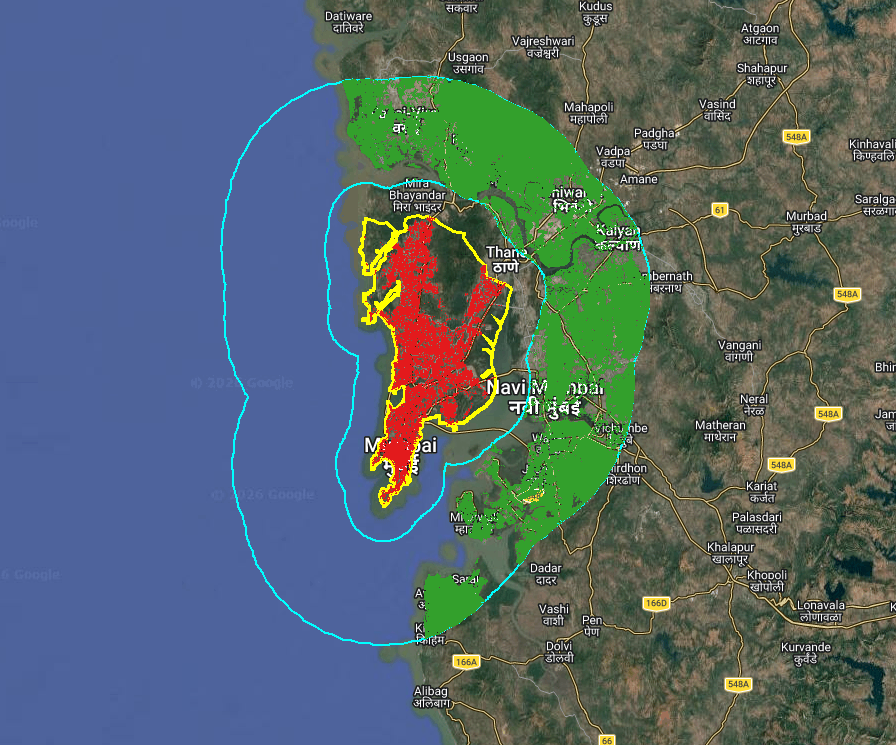
\includegraphics[width=0.75\textwidth]{zones_map_gee.png}
\caption{Urban zone (red), rural ring (green), district boundary
(yellow), outer edge of the ring (cyan). The western half of the ring
is open sea and drops out once water is excluded.}
\label{fig:zones}
\end{figure}

\paragraph{Classes that are neither clearly urban nor clearly rural.}
Three WorldCover classes are neither clearly urban nor clearly rural.
Herbaceous wetland (90) and mangrove (95) were excluded from the rural
reference: Mumbai's creeks are mangrove-lined and tidally inundated, so
these surfaces hold standing water for much of the tidal cycle and
behave thermally like water rather than land. They were not moved into
the urban zone either, since they are not built. Moss and lichen (100)
and snow and ice (70) do not occur in the study area. Bare and sparse
vegetation (60) was kept in the rural reference: it is genuinely
non-built, and excluding it would have biased the reference toward
vegetated, and therefore cooler, surfaces.

\paragraph{Water and wetland exclusion.}
\label{sec:waterexcl}

Permanent water (class 80) was removed from both zones.

\begin{table}[htbp]
\centering
\begin{tabular}{lrr}
\toprule
\textbf{Cover} & \textbf{Area (\si{\kilo\metre\squared})} & \textbf{Share} \\
\midrule
Permanent water (80)          & 1534.65 & 55.1\,\% \\
Wetland and mangrove (90, 95) &   73.64 &  2.6\,\% \\
Built-up (50)                 &  214.63 &  7.7\,\% \\
Usable rural cover            &  962.13 & 34.5\,\% \\
\midrule
Ring total                    & 2785.04 & 100\,\% \\
\bottomrule
\end{tabular}
\caption{Composition of the \SIrange{5}{20}{\kilo\metre} rural ring.
Over half is sea.}
\label{tab:ringcomp}
\end{table}

The reason is physical. Water has very high heat capacity and thermal
inertia, so its surface temperature barely moves over the diurnal
cycle while land swings widely. Leaving it in would anchor the rural
mean to a surface that cannot respond to the forcing being measured.

The bias would also change sign between day and night: the sea is
cooler than land by day, which would inflate daytime UHI, and warmer
by night, which would suppress night-time UHI. Section~\ref{sec:watertest}
measures this rather than assuming it.

% =============================================================
\section{Part A --- Day and night UHI from Landsat}
\label{sec:partA}
% =============================================================

\subsection{Method}

\begin{table}[htbp]
\centering
\small
\begin{tabular}{lll}
\toprule
 & \textbf{Daytime} & \textbf{Night-time} \\
\midrule
Scene   & \texttt{LC08\_148047\_20151008}
        & \texttt{LC08\_018197\_20151009} \\
Date    & 8 October 2015 & 9 October 2015 \\
Collection & \texttt{LANDSAT/LC08/C02/T1\_L2}
           & \texttt{LANDSAT/LC08/C02/T2} \\
Level   & Level-2 (surface temperature) & Level-1 (radiance) \\
Band    & \texttt{ST\_B10} & \texttt{B10} \\
Cloud cover & 8.49\,\% & \TODO{from M} \\
Valid-pixel fraction & \TODO{from M} & \TODO{from M} \\
\bottomrule
\end{tabular}
\caption{Landsat scenes used in Part~A.}
\label{tab:scenes}
\end{table}

The two scenes are one day apart, which is what makes the day/night
comparison meaningful --- a larger gap would mix the diurnal signal
with changing weather.

Night-time Landsat acquisitions are rare and irregular. They are
ascending-node passes, so the same ground location carries a different
WRS-2 path/row by night than by day, and they are frequently filed in
Tier~2 rather than Tier~1 because of looser geometric accuracy. Both
tiers were therefore searched.

\TODO{From M: why this pair and not another. What other candidates
were found, and why were they rejected? M's notes mention a November
pair whose night-time temperatures were anomalously low --- that is
exactly the kind of reasoning the brief is asking for, so write it up.
Also give the valid-pixel fraction over the AOI for both scenes.}

\paragraph{Cloud masking.}

Both scenes were screened on \texttt{QA\_PIXEL}, masking bits 0--5:
fill, dilated cloud, cirrus, cloud, cloud shadow and snow. Bit~6
(clear) and bit~7 (water) were left unmasked --- water is handled
through WorldCover instead, so that the two parts treat it the same
way.

\TODO{Report the fraction of the AOI that survived masking, for each
scene. The brief asks for this explicitly. Also note the known problem
with night-time screening: Fmask keys off the reflective bands, which
carry no signal on a night pass, so \texttt{QA\_PIXEL} is unreliable
at night. Say what you did about it and how much of the night AOI
survived.}

\paragraph{From radiance to temperature.}

\paragraph{Daytime.} The Collection~2 Level-2 product supplies surface
temperature directly. \texttt{ST\_B10} was scaled by \num{0.00341802}
with an offset of \num{149.0} to give kelvin, then converted to
Celsius. The USGS single-channel retrieval behind this product applies
its own emissivity correction, derived from ASTER GED.

\paragraph{Night-time.} No Level-2 surface temperature is produced for
night acquisitions, so the Level-1 product was used. Band~10 digital
numbers were converted to spectral radiance using the scene's own
\texttt{RADIANCE\_MULT\_BAND\_10} and \texttt{RADIANCE\_ADD\_BAND\_10},
then inverted through the Planck function with
$K_1 = \num{774.8853}$ and $K_2 = \num{1321.0789}$:

\begin{equation}
  T_b = \frac{K_2}{\ln\!\left(\dfrac{K_1}{L_\lambda} + 1\right)}
\end{equation}

\paragraph{The night-time figure is brightness temperature, not LST.}
No emissivity correction was applied to the night scene, so what
Part~A reports at night is $T_b$. Brightness temperature is lower than
land surface temperature wherever $\varepsilon < 1$, and the offset
differs between built-up ($\varepsilon \approx 0.97$) and vegetated
($\varepsilon \approx 0.98$--$0.99$) surfaces, so it does not cancel
in the urban-minus-rural subtraction. This matters when the night
figures are compared against MODIS in Section~\ref{sec:comparison},
where MODIS night LST \emph{is} emissivity-corrected.

\TODO{The brief lists emissivity as a scored decision point and asks
what applying it changed. Two options. Either apply a class-based
emissivity correction to the night scene --- WorldCover class to
$\varepsilon$, then
$T_s = T_b / [1 + (\lambda T_b / c_2)\ln\varepsilon]$ --- and report
both $T_b$ and $T_s$ so the difference is visible; or keep $T_b$ and
justify the choice, stating the expected size and direction of the
error. The first is stronger and is about ten lines of code. Either
way, say plainly which you did.}

\paragraph{Statistics scale.}
\label{sec:landsat_scale}

The analysis extent --- the district plus the \SI{20}{\kilo\metre}
rural buffer --- covers about \SI{2800}{\kilo\metre\squared}, which at
the native \SI{30}{\metre} is roughly \num{3.1} billion pixels and
beyond what Earth Engine will reduce interactively. Zonal statistics
were computed at \SI{100}{\metre}, diagnostics at
\SIrange{200}{300}{\metre}, and raster exports left at
\SI{30}{\metre}. At \SI{100}{\metre} the Landsat statistics are still
ten times finer than the MODIS grid, so the resolution argument in
Section~\ref{sec:comparison} is unaffected. The boundary was also
simplified to a \SI{100}{\metre} tolerance before the ring was built;
Part~B uses the unsimplified polygon, so the two rings differ by at
most \SI{100}{\metre} --- sub-pixel for both.

\subsection{Results}

\begin{table}[htbp]
\centering
\begin{tabular}{lrrrr}
\toprule
\textbf{Variable} & \textbf{Urban} & \textbf{Rural} &
\textbf{UHI} & $n_{\mathrm{urb}}$ \\
 & (\si{\degreeCelsius}) & (\si{\degreeCelsius}) &
(\si{\degreeCelsius}) & \\
\midrule
Day LST (L2 product)      & \TODO{} & \TODO{} & 2.39 & \TODO{} \\
Night $T_b$ (no correction) & \TODO{} & \TODO{} & 1.15 & \TODO{} \\
Night LST (class $\varepsilon$) & \TODO{} & \TODO{} & 2.13 & \TODO{} \\
\bottomrule
\end{tabular}
\caption{Landsat UHI, 8--9 October 2015, external
\SIrange{5}{20}{\kilo\metre} rural ring. \TODO{fill urban/rural means
and pixel counts from \texttt{Mumbai\_Landsat\_UHI\_headline\_v2.csv}}}
\label{tab:landsat_uhi}
\end{table}

Day and night UHI are close in magnitude: \SI{2.39}{\degreeCelsius}
and \SI{2.13}{\degreeCelsius}. Valid-pixel fractions after QA masking
were 88.0\,\% over the city and 95.2\,\% over the ring for the day
scene, and 100\,\% and 99.6\,\% for the night scene.

The night figure should be read with care. Fmask keys off the
reflective bands, which carry no signal on a night pass, so a
near-perfect night valid fraction reflects the mask finding nothing to
flag rather than a genuinely clear scene.

\TODO{Insert the LST map, anomaly map and distribution plot --- the
brief requires all three, for day and night. Rasters are exported in
\texttt{Mumbai\_UHI\_Landsat}; they need rendering with a scale bar,
north arrow, and a shared colour scale between day and night.}

\TODO{Interpret the day/night result. Points worth working through:

(i) Day and night UHI are nearly equal here
(2.39 against 2.13\,\si{\degreeCelsius}), whereas Part~B finds
day and night differ sharply by season. What does a single October
scene capture that a seasonal mean does not, and vice versa?

(ii) Compare against Part~B's post-monsoon 2015 Terra figures
(Table~\ref{tab:comparison}): night 2.09 against your 2.13 is close
agreement between two independent sensors; day 1.24 against 2.39 is
not. Which of the two is the more surprising and why?

(iii) The night distribution in the histogram is strongly
right-shifted for urban while the day distributions overlap heavily.
What does that say about how uniformly the city is warmer at each time
of day?}

% =============================================================
\section{Part B --- Seasonal UHI from MODIS}
\label{sec:partB}
% =============================================================

\subsection{Method}

Seasonal LST comes from the MODIS eight-day composites,
\texttt{MODIS/061/MOD11A2} (Terra) \citep{mod11a2} and
\texttt{MODIS/061/MYD11A2} (Aqua) \citep{myd11a2}, both at
\SI{1}{\kilo\metre}. These are Collection~6.1 split-window retrievals
with land-cover-based emissivity.

The eight-day product was chosen over the daily one
(\texttt{MOD11A1}/\texttt{MYD11A1}) because the daily product leaves
every cloud gap to be handled by hand, and Mumbai has four months of
near-continuous monsoon cloud. The eight-day product applies a
consistent clear-sky selection instead. The cost is that it hides how
few days actually contributed, which is measured in
Section~\ref{sec:sampling}.

\paragraph{Terra and Aqua.}
Both platforms were used rather than one. Terra crosses at about
\texttt{10:30} and \texttt{22:30} local solar time; Aqua at about
\texttt{13:30} and \texttt{01:30}. Terra's morning pass is close to
Landsat~8's ($\approx$\texttt{10:30}), so the Terra daytime numbers
are the ones comparable with Part~A. Aqua sits nearer the daily
maximum and the pre-dawn minimum, so it better captures the true
extremes. The Terra--Aqua gap within a season isolates time of day
from season.

Observation times were read from the \texttt{Day\_view\_time} and
\texttt{Night\_view\_time} bands rather than assumed. Over the urban
zone they average \textbf{10:38} and \textbf{22:14} for Terra, and
\textbf{13:28} and \textbf{01:52} for Aqua. Terra's morning pass is
within about eight minutes of Landsat's.

\paragraph{Season definition.}

\begin{table}[htbp]
\centering
\begin{tabular}{lll}
\toprule
\textbf{Season} & \textbf{Months} & \textbf{Role} \\
\midrule
Winter               & January--February & Seasonal contrast \\
Pre-monsoon (summer) & March--May        & Seasonal contrast \\
Southwest monsoon    & June--September   & Seasonal contrast \\
Post-monsoon         & October--December & Landsat comparison \\
\bottomrule
\end{tabular}
\caption{India Meteorological Department four-season classification
\citep{imd_seasons}. All four were computed.}
\label{tab:seasons}
\end{table}

The brief asks for two or three seasons; the first three cover the
full range of surface moisture and insolation in Mumbai. Post-monsoon
was added because the Landsat pair falls in it, so the cross-sensor
comparison in Section~\ref{sec:comparison} has a matching season.

\paragraph{Why IMD and not DJF/MAM/JJA.}
December--January--February for winter is a mid-latitude convention
and does not describe a tropical monsoon coast. Mumbai's year is set
by the onset and withdrawal of the southwest monsoon, not the
solstices. December still carries post-monsoon soil moisture and is
not thermally like January, which is why IMD places it in
post-monsoon. And no IMD season crosses a calendar year, so each year
gives exactly one clean instance of each season --- which is what
makes the year-by-year analysis in Section~\ref{sec:interannual}
possible. A DJF winter would straddle two years and force an arbitrary
choice about each December.

\paragraph{Climatological basis.}
\TODO{Two or three sentences on Mumbai's climate with a real citation:
mean monthly temperature and rainfall, and normal monsoon onset and
withdrawal dates. IMD Climatological Tables or the IMD Mumbai regional
page. This is what turns the season definition from an assertion into
a defended choice. Without it this section loses marks.}

\paragraph{Quality screening.}
\label{sec:qc}

Pixels were screened on \texttt{QC\_Day} and \texttt{QC\_Night}, keeping
mandatory QA (bits 0--1) of 0 or 1 --- not cloud-flagged, not otherwise
unproduced --- and LST error (bits 6--7) of 2 or better, meaning an
average retrieval error at or below \SI{3}{\kelvin}.

The eight-day product is already cloud-screened, so this is not cloud
masking. It removes retrievals produced under marginal conditions with
large stated errors, which in a monsoon climate cluster in the season
of most interest.

A stricter setting (mandatory QA $=0$, LST error
$\leq\,$\SI{2}{\kelvin}) was tried first and emptied some night-time
zones entirely, producing null zonal means. The relaxed setting was
used throughout. Pixel counts never fall below 239 urban and 917
rural.

\paragraph{Compositing.}
LST bands were scaled by \num{0.02} to kelvin, then
\SI{273.15}{\kelvin} subtracted. View-time bands were scaled by
\num{0.1} to local solar hours. For each platform, mode and season,
all qualifying composites from 2019--2023 were averaged per pixel.
Zonal means were taken at \SI{1000}{\metre}, the native MODIS grid
spacing, so no resampling precedes the statistics.

\begin{equation}
  \mathrm{UHI} = \overline{T_{\mathrm{urban}}} - \overline{T_{\mathrm{rural}}}
\end{equation}

The urban zone holds 241 valid pixels at \SI{1}{\kilo\metre} and the
rural zone 917--1055. The urban count is the binding constraint on
precision.

\subsection{Results}

\begin{table}[htbp]
\centering
\small
\begin{tabular}{llrrrrrr}
\toprule
\textbf{Platform} & \textbf{Season} & \textbf{Obs.} &
\textbf{Urban} & \textbf{Rural} & \textbf{UHI} &
$n_{\mathrm{urb}}$ & $n_{\mathrm{rur}}$ \\
 & & \textbf{time} & (\si{\degreeCelsius}) & (\si{\degreeCelsius}) &
(\si{\degreeCelsius}) & & \\
\midrule
\multicolumn{8}{l}{\textit{Daytime}} \\
Terra & Winter       & 10:38 & 32.10 & 32.50 & $-0.41$ & 241 & 1055 \\
Terra & Pre-monsoon  & 10:37 & 36.38 & 39.10 & $-2.72$ & 241 & 1055 \\
Terra & Monsoon      & 10:40 & 31.16 & 31.09 & $+0.07$ & 241 & 1055 \\
Terra & Post-monsoon & 10:32 & 32.62 & 30.96 & $+1.67$ & 241 & 1055 \\
Aqua  & Winter       & 13:27 & 35.68 & 36.55 & $-0.87$ & 241 & 1055 \\
Aqua  & Pre-monsoon  & 13:28 & 39.60 & 42.24 & $-2.64$ & 241 & 1055 \\
Aqua  & Monsoon      & 13:31 & 32.99 & 32.07 & $+0.92$ & 241 & 1055 \\
Aqua  & Post-monsoon & 13:32 & 34.94 & 33.27 & $+1.67$ & 241 & 1055 \\
\midrule
\multicolumn{8}{l}{\textit{Night-time}} \\
Terra & Winter       & 22:14 & 22.23 & 19.43 & $+2.80$ & 239 &  917 \\
Terra & Pre-monsoon  & 22:14 & 26.20 & 24.30 & $+1.90$ & 241 &  977 \\
Terra & Monsoon      & 22:08 & 22.78 & 21.05 & $+1.73$ & 241 & 1055 \\
Terra & Post-monsoon & 22:09 & 24.51 & 22.13 & $+2.38$ & 241 & 1042 \\
Aqua  & Winter       & 01:50 & 21.28 & 19.03 & $+2.25$ & 241 & 1016 \\
Aqua  & Pre-monsoon  & 01:52 & 25.64 & 23.11 & $+2.53$ & 241 & 1012 \\
Aqua  & Monsoon      & 01:55 & 22.30 & 20.92 & $+1.38$ & 241 & 1055 \\
Aqua  & Post-monsoon & 01:53 & 23.61 & 21.14 & $+2.47$ & 241 & 1055 \\
\bottomrule
\end{tabular}
\caption{Seasonal surface UHI intensity, 2019--2023 means.}
\label{tab:headline}
\end{table}

\begin{figure}[htbp]
\centering
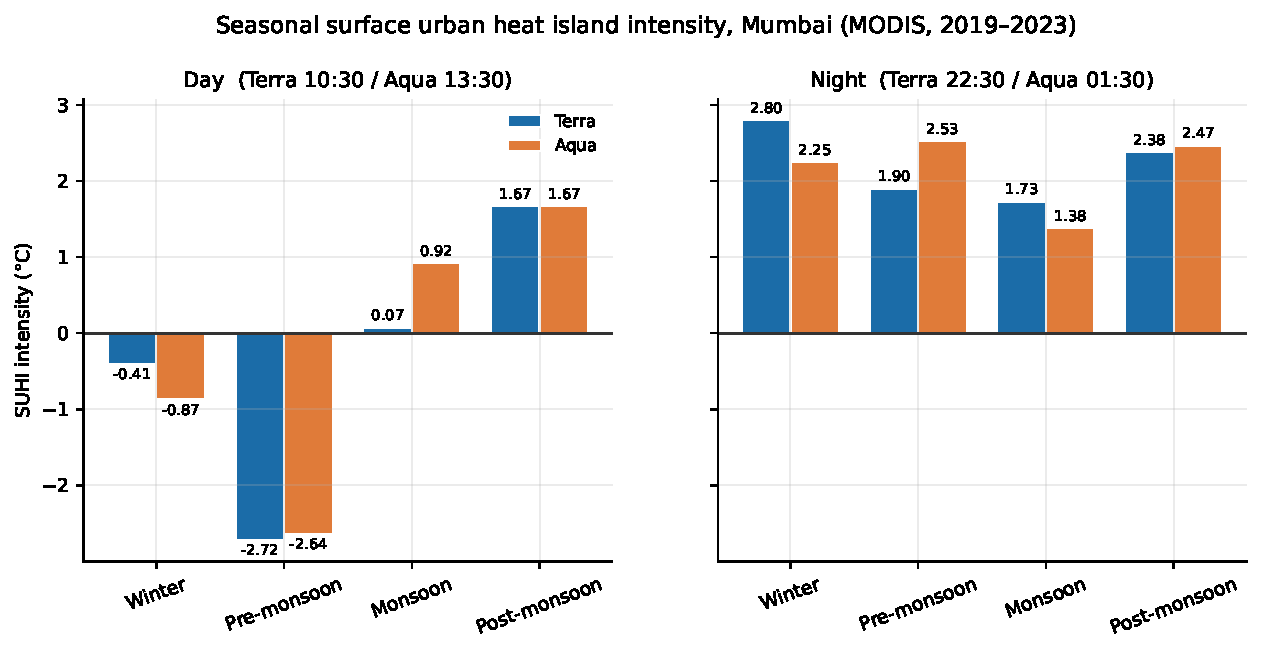
\includegraphics[width=\textwidth]{fig1_seasonal_suhi.pdf}
\caption{Seasonal SUHI, both platforms, day and night.}
\label{fig:seasonal}
\end{figure}

\begin{figure}[htbp]
\centering
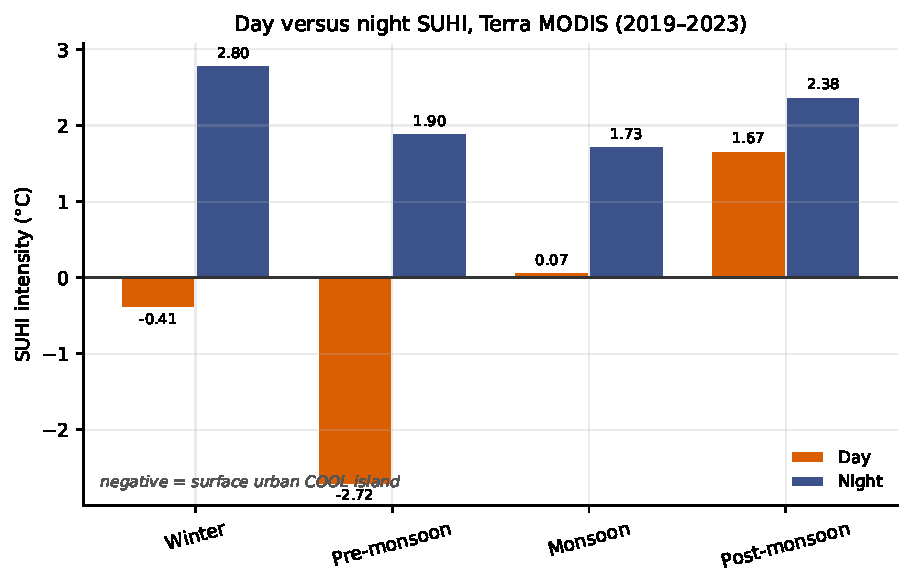
\includegraphics[width=0.78\textwidth]{fig2_day_vs_night.pdf}
\caption{Day and night SUHI side by side, Terra.}
\label{fig:daynight}
\end{figure}

Night-time UHI is positive in every season on both platforms, from
\SI{+1.38}{\degreeCelsius} to \SI{+2.80}{\degreeCelsius}. Daytime UHI
is negative in winter ($-0.41$ Terra, $-0.87$ Aqua) and strongly
negative in pre-monsoon ($-2.72$, $-2.64$), near zero in monsoon, and
positive only in post-monsoon ($+1.67$ on both). A negative value
means the rural surface is hotter than the urban one --- a surface
urban \emph{cool} island.

\TODO{Interpret. This is the main result and carries the most marks,
so it needs several paragraphs of reasoning, not a restatement of the
table. Work through at least:

(i) Why is daytime UHI negative in winter and pre-monsoon? Compare the
means separately first --- in pre-monsoon urban is 36.38 and rural
39.10, so the city has not cooled, the countryside has heated. Which
thermal property from the lecture material explains a dry bare surface
heating faster than a built one? Thermal inertia and heat capacity are
the relevant ones, and the Class-4 table compares water, sand,
vegetation and urban directly.

(ii) Why is night-time UHI positive in every season when daytime is
not? Connect to Oke's point that UHI is mostly nocturnal, and to
built-up surfaces releasing stored heat after sunset.

(iii) Monsoon daytime UHI is near zero (+0.07 Terra, +0.92 Aqua).
What happens to the urban--rural contrast when both surfaces are wet
and evaporating? Note the sampling bias in
Section~\ref{sec:sampling} compromises this reading and say so.

(iv) Terra and Aqua disagree most in monsoon daytime (0.85 apart) and
pre-monsoon night (0.63 apart). The only difference is three hours of
clock time --- what does that gap say about how fast the surface is
changing at those hours?}

\paragraph{The day--night reversal.}
Daytime UHI is negative in two of four seasons while night-time UHI is
positive in all four. \TODO{This is the strongest single finding in
the report and should be drawn out here in a short paragraph: it is
the nocturnal dominance described by Oke appearing in your own
measurements, and it links Part~B directly to Part~A's day/night
contrast. Two supporting calculations are available from
Table~\ref{tab:headline} if you want them --- urban minus rural
diurnal range per zone, and mean LST by land-cover class.}

\subsection{Clear-sky sampling bias}
\label{sec:sampling}

The monsoon composite is not an average over the monsoon. It averages
those monsoon days clear enough for a retrieval to be produced and
pass screening --- the least monsoon-like days of the season.

\begin{table}[htbp]
\centering
\begin{tabular}{lrrr}
\toprule
\textbf{Season} & \textbf{Composites} & \textbf{Mean valid} &
\textbf{Retention} \\
 & \textbf{available} & \textbf{retrievals} & \\
\midrule
Winter       & 40 & 15.6 & 38.9\,\% \\
Pre-monsoon  & 55 & 21.2 & 38.6\,\% \\
Monsoon      & 80 & 10.7 & 13.3\,\% \\
Post-monsoon & 55 & 20.4 & 37.1\,\% \\
\bottomrule
\end{tabular}
\caption{Valid retrievals per pixel against composites available,
Terra day, 2019--2023.}
\label{tab:sampling}
\end{table}

\begin{figure}[htbp]
\centering
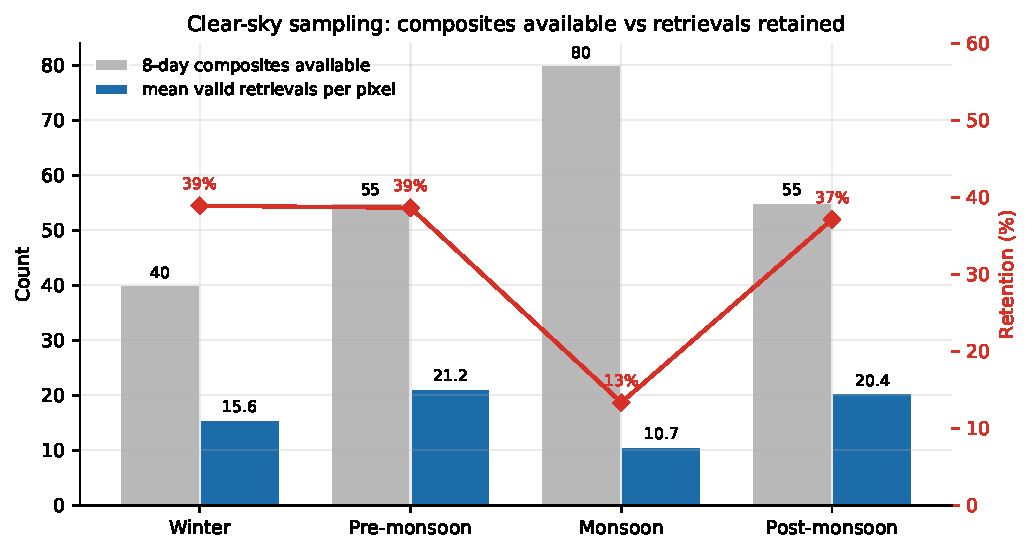
\includegraphics[width=0.78\textwidth]{fig8_sampling_bias.pdf}
\caption{Composites available against retrievals retained. Monsoon has
the most input and the fewest usable observations.}
\label{fig:sampling}
\end{figure}

Monsoon has twice as many composites available as winter but retains
the fewest valid retrievals --- 10.7 per pixel, 13.3\,\%, against
roughly 38\,\% elsewhere.

\TODO{Interpret. Say what the monsoon number therefore represents, and
in which direction it biases the monsoon UHI --- if the only usable
monsoon days are the clearer, brighter ones, is the retrieved monsoon
UHI too high or too low against a true monsoon average? Then say how
much weight the monsoon row deserves.}

\subsection{Urban and rural distributions}

\begin{figure}[htbp]
\centering
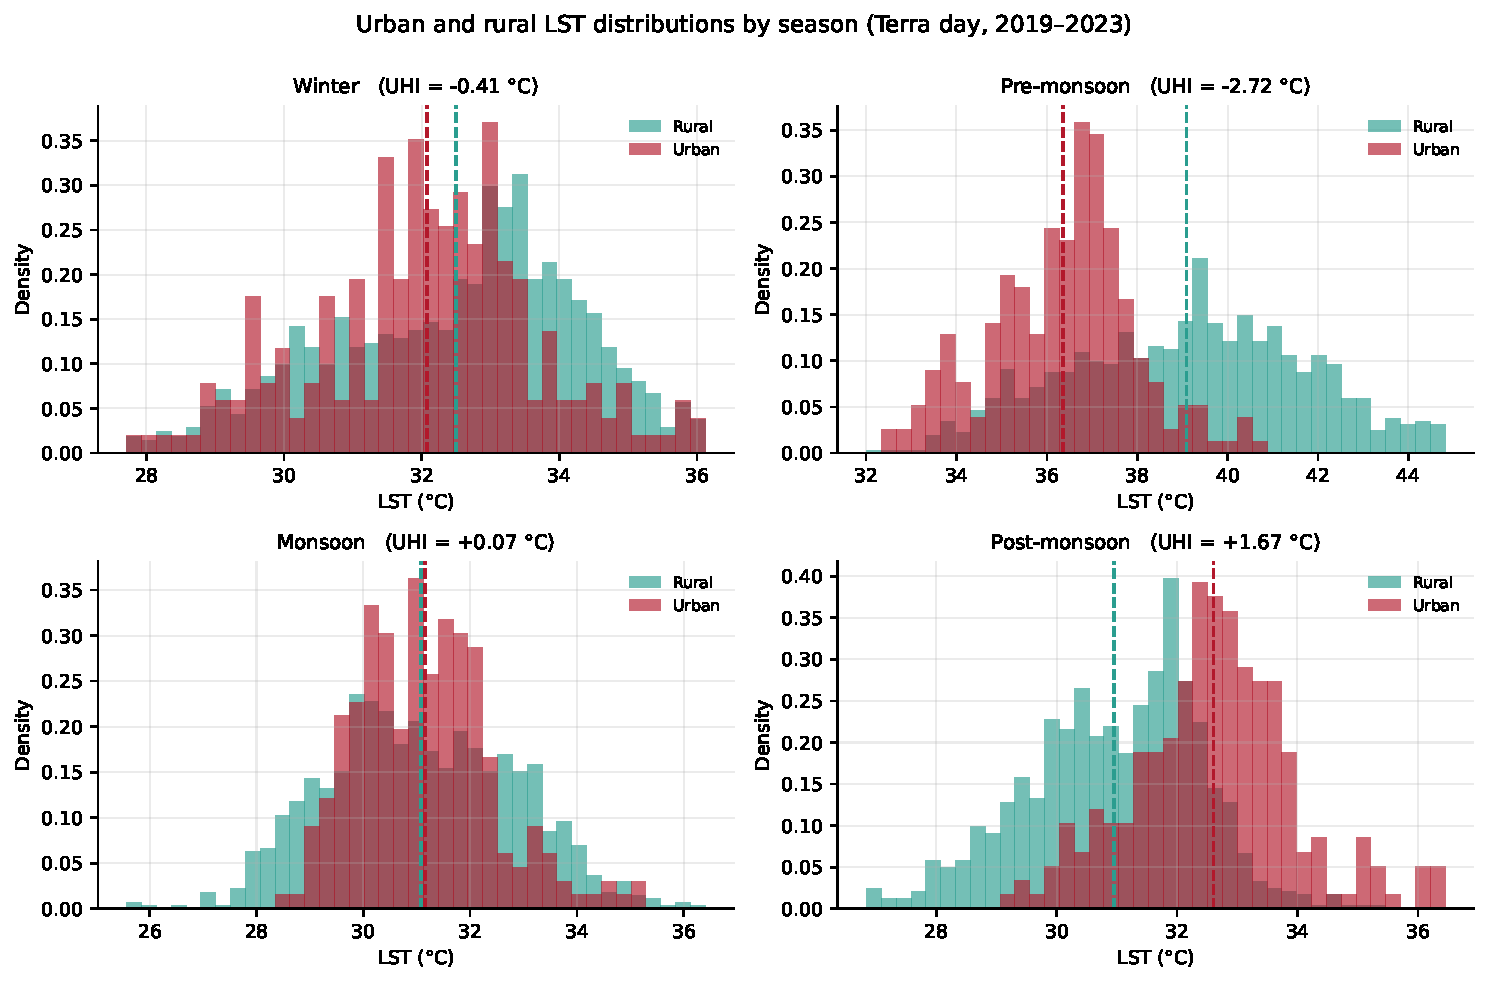
\includegraphics[width=\textwidth]{fig6_distributions.pdf}
\caption{Urban and rural LST distributions by season, Terra day.
Dashed lines mark zone means.}
\label{fig:dist}
\end{figure}

\TODO{Interpret. Pre-monsoon shows the two distributions almost fully
separated with rural to the right of urban; post-monsoon reverses with
a smaller gap; winter and monsoon overlap heavily. Address whether the
zones separate or merely shift, and note that the rural distribution
is consistently wider (rural sd 1.43--3.02 against urban 1.24--1.60)
--- what does that say about how mixed the rural zone is?}

% =============================================================
\section{Sensitivity analysis}
\label{sec:sensitivity}
% =============================================================

\subsection{Interannual stability (Part B)}
\label{sec:interannual}

\begin{table}[htbp]
\centering
\begin{tabular}{lrrrrrr}
\toprule
\textbf{Season} & \textbf{2019} & \textbf{2020} & \textbf{2021} &
\textbf{2022} & \textbf{2023} & \textbf{Range} \\
\midrule
Winter       & $-1.25$ & $-0.27$ & $-0.38$ & $+0.17$ & $-0.30$ & 1.42 \\
Pre-monsoon  & $-3.27$ & $-2.92$ & $-2.74$ & $-2.22$ & $-2.45$ & 1.06 \\
Monsoon      & $+0.06$ & $+1.45$ & $-0.39$ & $-0.31$ & $-0.76$ & 2.20 \\
Post-monsoon & $+1.78$ & $+1.59$ & $+2.01$ & $+1.54$ & $+1.41$ & 0.60 \\
\bottomrule
\end{tabular}
\caption{UHI (\si{\degreeCelsius}) by season and year, Terra day.}
\label{tab:interannual}
\end{table}

\begin{figure}[htbp]
\centering
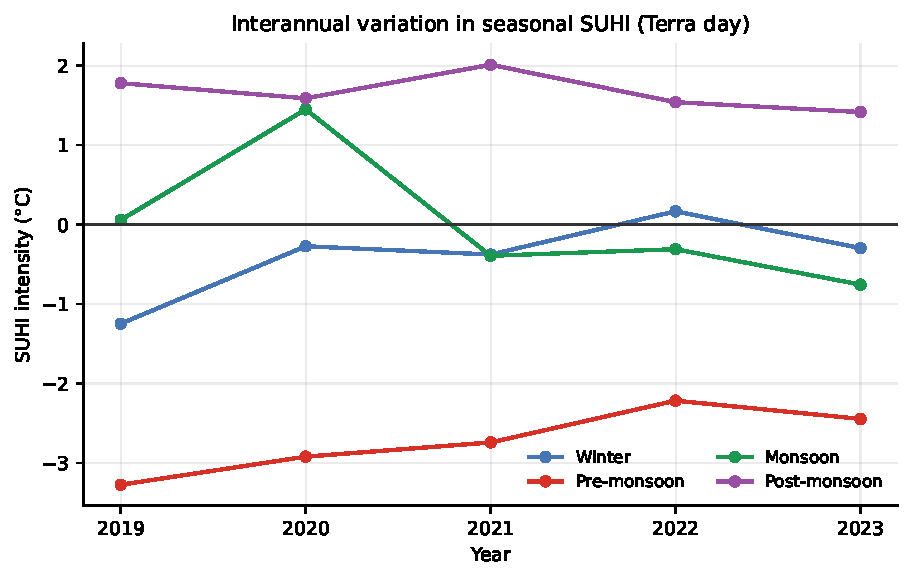
\includegraphics[width=0.78\textwidth]{fig3_interannual.pdf}
\caption{Year-by-year seasonal SUHI, Terra day.}
\label{fig:interannual}
\end{figure}

Pre-monsoon is negative in all five years and post-monsoon positive in
all five. Winter changes sign once (2022). Monsoon changes sign three
times and has the widest range, \SI{2.20}{\degreeCelsius}.

\TODO{Interpret. The question is not whether the numbers move but
whether the seasonal ordering holds every year --- check and state it.
Then compare the interannual ranges against the between-season
differences: pre-monsoon and post-monsoon are about
4.4\,\si{\degreeCelsius} apart with year-to-year ranges of
1.06 and 0.60, whereas monsoon's range of 2.20 is larger than its
distance from zero. Say which seasonal results you would stand behind
and which you would not, and tie the monsoon instability back to
Section~\ref{sec:sampling}.}

\subsection{Rural ring definition (Part B)}
\label{sec:ringsens}

\begin{table}[htbp]
\centering
\begin{tabular}{lrrrrr}
\toprule
\textbf{Ring} & \textbf{Winter} & \textbf{Pre-mon.} &
\textbf{Monsoon} & \textbf{Post-mon.} & $n_{\mathrm{rur}}$ \\
\midrule
\SIrange{2}{20}{\kilo\metre}  & $-0.29$ & $-2.55$ & $+0.16$ & $+1.73$ & 1115 \\
\SIrange{5}{20}{\kilo\metre}$^\dagger$ & $-0.41$ & $-2.72$ & $+0.07$ & $+1.67$ & 1055 \\
\SIrange{10}{25}{\kilo\metre} & $-0.58$ & $-3.05$ & $-0.05$ & $+1.65$ &  893 \\
\SIrange{5}{30}{\kilo\metre}  & $-0.40$ & $-2.74$ & $+0.09$ & $+1.70$ & 1055 \\
\midrule
\textbf{Range}                &   0.29  &   0.50  &   0.21  &   0.08  & \\
\bottomrule
\end{tabular}
\caption{UHI (\si{\degreeCelsius}) under four rural ring definitions,
Terra day. $^\dagger$ headline definition.}
\label{tab:ringsens}
\end{table}

\begin{figure}[htbp]
\centering
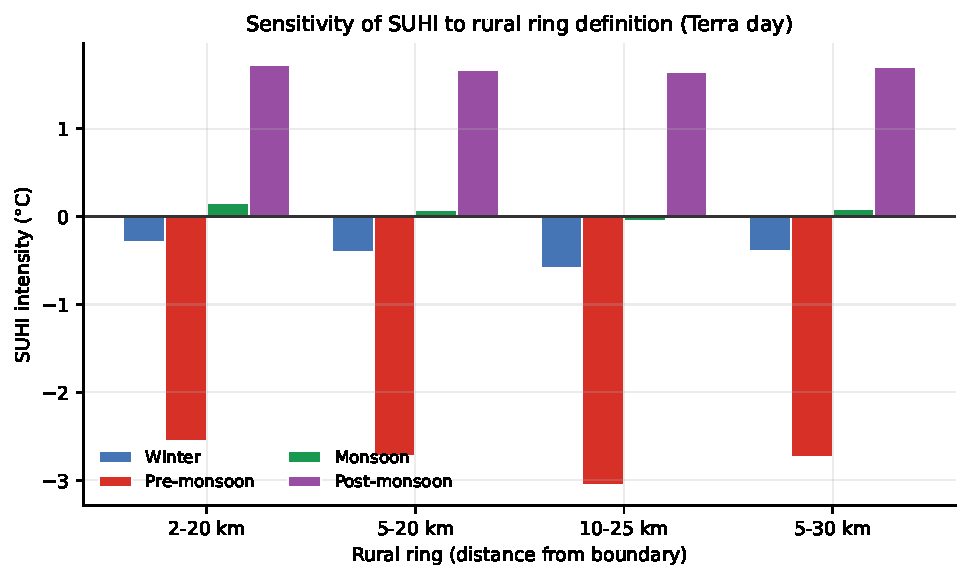
\includegraphics[width=0.82\textwidth]{fig4_ring_sensitivity.pdf}
\caption{SUHI under four rural ring definitions.}
\label{fig:ring}
\end{figure}

Moving the inner edge from \SI{2}{\kilo\metre} to
\SI{10}{\kilo\metre} shifts UHI by up to
\SI{0.50}{\degreeCelsius}. Pushing the outer edge from
\SI{20}{\kilo\metre} to \SI{30}{\kilo\metre} changes almost nothing
(\num{0.01} to \SI{0.03}{\degreeCelsius}).

\TODO{Interpret. Two things. First, direction: as the inner edge moves
outward the rural mean rises and UHI becomes more negative in every
season --- what does a rural reference that keeps getting hotter with
distance imply about how far the city's influence reaches, and does
that support or undermine the 5\,km gap? Second, the outer edge barely
matters while the inner edge does; what does that asymmetry say about
where the useful rural land sits? Then compare against M's sweep in
Section~\ref{sec:landsatsens} and explain any difference in terms of
pixel size.}

\subsection{Water in the rural reference (Part B)}
\label{sec:watertest}

UHI was recomputed with water, wetland and mangrove left in the rural
reference, everything else fixed.

\begin{table}[htbp]
\centering
\small
\begin{tabular}{llrrr}
\toprule
\textbf{Mode} & \textbf{Season} & \textbf{Water excl.} &
\textbf{Water incl.} & \textbf{Difference} \\
\midrule
Day   & Winter       & $-0.41$ & $-0.12$ & $+0.291$ \\
Day   & Pre-monsoon  & $-2.72$ & $-2.28$ & $+0.445$ \\
Day   & Monsoon      & $+0.07$ & $+0.25$ & $+0.176$ \\
Day   & Post-monsoon & $+1.67$ & $+1.77$ & $+0.104$ \\
\midrule
Night & Winter       & $+2.80$ & $+2.80$ & $-0.004$ \\
Night & Pre-monsoon  & $+1.90$ & $+1.93$ & $+0.031$ \\
Night & Monsoon      & $+1.73$ & $+1.64$ & $-0.087$ \\
Night & Post-monsoon & $+2.38$ & $+2.35$ & $-0.035$ \\
\bottomrule
\end{tabular}
\caption{Effect of retaining water in the rural reference, Terra.
All values \si{\degreeCelsius}.}
\label{tab:watertest}
\end{table}

\begin{figure}[htbp]
\centering
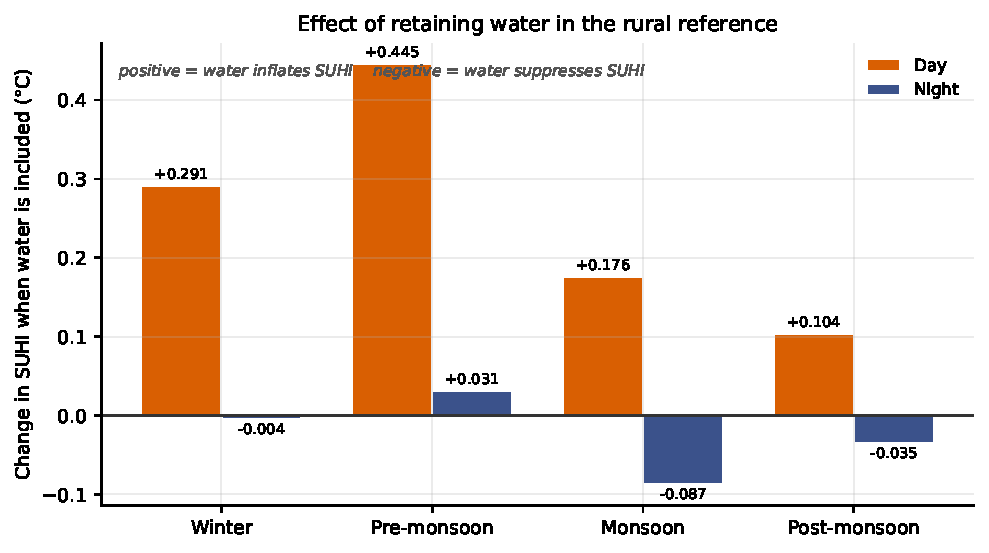
\includegraphics[width=0.82\textwidth]{fig5_water_test.pdf}
\caption{Change in SUHI when water is retained in the rural zone.}
\label{fig:water}
\end{figure}

Every daytime difference is positive (\num{+0.10} to \num{+0.45}).
Three of four night-time differences are negative
(\num{-0.004} to \num{-0.087}).

\TODO{Interpret, tying back to Section~\ref{sec:waterexcl}. The
prediction was that including water inflates daytime UHI and
suppresses night-time UHI, because the sea is cooler than land by day
and warmer by night. State whether the signs bear that out. Then note
the daytime effect is roughly five times the night-time one and
explain why --- what is the sea's diurnal temperature range compared
with land's? Finally, would an error this size have changed any
conclusion in Section~\ref{sec:partB}?}

\subsection{Reference definition and emissivity (Part A)}
\label{sec:landsatsens}

\paragraph{Rural ring.}
The same four ring variants used in Part~B were run on the Landsat
scenes.

\begin{table}[htbp]
\centering
\begin{tabular}{lrr}
\toprule
\textbf{Ring} & \textbf{Day UHI} & \textbf{Night UHI} \\
 & (\si{\degreeCelsius}) & (\si{\degreeCelsius}) \\
\midrule
\SIrange{2}{20}{\kilo\metre}  & 2.400 & 2.047 \\
\SIrange{5}{20}{\kilo\metre}$^\dagger$ & 2.385 & 2.127 \\
\SIrange{10}{25}{\kilo\metre} & 2.443 & 2.223 \\
\SIrange{5}{30}{\kilo\metre}  & 2.392 & 2.129 \\
\midrule
\textbf{Range}                & 0.058 & 0.176 \\
\bottomrule
\end{tabular}
\caption{Landsat UHI under four rural ring definitions.
$^\dagger$ headline definition.}
\label{tab:landsat_ring}
\end{table}

Landsat UHI moves by at most \SI{0.18}{\degreeCelsius} across the four
rings --- markedly less than the MODIS equivalent in
Table~\ref{tab:ringsens}, which ranges up to
\SI{0.50}{\degreeCelsius}.

\TODO{Interpret. Why would the finer sensor be \emph{less} sensitive
to where the rural ring sits? Consider what a \SI{1}{\kilo\metre}
pixel does at the ring's inner edge that a \SI{100}{\metre} pixel does
not, and whether the seasonal composite in Part~B samples a different
set of surfaces than a single October scene.}

\paragraph{Emissivity correction.}
Night-time UHI computed from brightness temperature is
\SI{1.15}{\degreeCelsius}; from emissivity-corrected LST it is
\SI{2.13}{\degreeCelsius}. Applying the correction nearly doubles the
result.

The correction does not cancel in the urban-minus-rural subtraction
because the two zones have different emissivities: built-up is
assigned \num{0.970} and vegetated surfaces \num{0.985}. A surface
with lower emissivity emits less at a given temperature, so correcting
for it raises the retrieved temperature more over the city than over
the countryside, widening the difference.

\TODO{Interpret, and connect to the lecture material: roughly
\SI{1}{\kelvin} of LST error per \SI{1.5}{\percent} of emissivity
error. Given a difference of \num{0.015} between the built and
vegetated values used here, is a shift of
\SI{0.98}{\degreeCelsius} the size you would expect? Then state
plainly which figure the report treats as its night-time result and
why.}

% =============================================================
\section{Comparing Landsat and MODIS}
\label{sec:comparison}
% =============================================================

The overlapping season is post-monsoon: the Landsat pair was acquired
8--9~October~2015.

\paragraph{Matching in time.}
The headline MODIS figures are 2019--2023 means; the Landsat
observation is a single day in 2015. Comparing them directly would mix
the sensor difference with eight years of urban growth and
year-to-year variation. Post-monsoon was therefore recomputed for 2015
alone. Both are given below: the gap between the two MODIS rows is
interannual variation, and the gap between the matched MODIS row and
the Landsat row is the sensor comparison proper.

\begin{table}[htbp]
\centering
\small
\begin{tabular}{lllrrr}
\toprule
\textbf{Sensor} & \textbf{Period} & \textbf{Mode} &
\textbf{Obs.\ time} & \textbf{Res.} & \textbf{UHI} \\
 & & & (local) & (\si{\metre}) & (\si{\degreeCelsius}) \\
\midrule
Landsat 8 & 8 Oct 2015 & Day   & 10:30 & 30 & $+2.39$ \\
Landsat 8 & 9 Oct 2015 & Night & 22:00 & 30 & $+2.13$ \\
\midrule
Terra & 2015     & Day   & 10:41 & 1000 & $+1.24$ \\
Terra & 2019--23 & Day   & 10:32 & 1000 & $+1.67$ \\
Aqua  & 2015     & Day   & 13:24 & 1000 & $+1.71$ \\
Aqua  & 2019--23 & Day   & 13:32 & 1000 & $+1.67$ \\
\midrule
Terra & 2015     & Night & 22:19 & 1000 & $+2.09$ \\
Terra & 2019--23 & Night & 22:09 & 1000 & $+2.38$ \\
Aqua  & 2015     & Night & 01:49 & 1000 & $+2.36$ \\
Aqua  & 2019--23 & Night & 01:53 & 1000 & $+2.47$ \\
\bottomrule
\end{tabular}
\caption{Post-monsoon UHI across both sensors. All rows use the same
\SIrange{5}{20}{\kilo\metre} rural ring. The Landsat night value is
emissivity-corrected LST. MODIS 2015 rows are matched to the Landsat
acquisition year. \TODO{confirm the Landsat overpass times from the
scene metadata}}
\label{tab:comparison}
\end{table}

\begin{figure}[htbp]
\centering
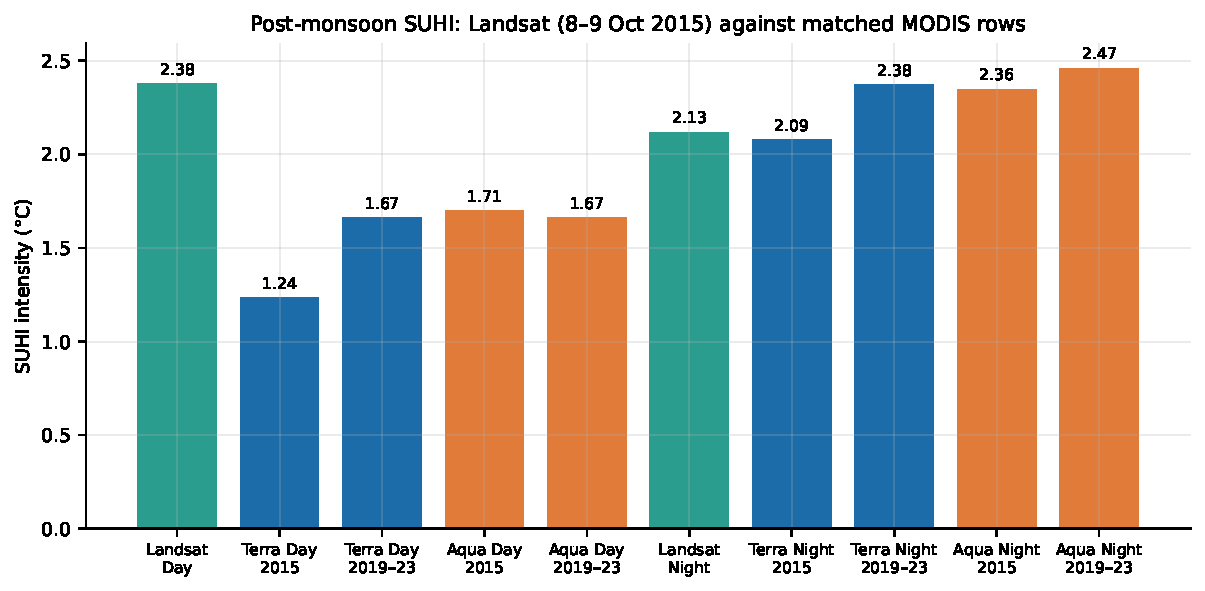
\includegraphics[width=0.82\textwidth]{fig7_cross_sensor.pdf}
\caption{MODIS post-monsoon SUHI, 2015 against the 2019--2023 mean.}
\label{fig:cross}
\end{figure}

\subsection{Reconciling the two parts}
\label{sec:zonemismatch}

An earlier version of Part~A used non-built pixels \emph{inside} the
city boundary as its rural reference, and did not exclude water. That
is a different definition from Part~B's external ring, and it made the
two parts non-comparable. Part~A was therefore rerun with the external
\SIrange{5}{20}{\kilo\metre} ring, water and wetland excluded, so both
parts now use identical zones.

The change is large enough to matter:

\begin{table}[htbp]
\centering
\begin{tabular}{lrrr}
\toprule
\textbf{Variable} & \textbf{Internal} & \textbf{External ring} &
\textbf{Change} \\
 & (\si{\degreeCelsius}) & (\si{\degreeCelsius}) &
(\si{\degreeCelsius}) \\
\midrule
Day LST     & 3.71 & 2.385 & $-1.33$ \\
Night $T_b$   & 0.32 & 1.146 & $+0.83$ \\
Night LST   & --- & 2.127 & --- \\
\bottomrule
\end{tabular}
\caption{Effect of moving the rural reference outside the city.
Internal-reference figures are from the earlier Part~A run.
\TODO{replace with the exact values in
\texttt{Mumbai\_Landsat\_ReferenceDefinition\_v2.csv}}}
\label{tab:refdef}
\end{table}

\TODO{Interpret. The night-time figure more than trebles when the
reference moves outside the city, while the daytime figure falls. Both
changes have the same cause --- an internal reference sits inside the
urban thermal plume --- but they move in opposite directions. Work out
why, remembering that daytime UHI in Part~B is driven by the rural
surface heating faster than the city, whereas night-time UHI is driven
by the city releasing stored heat. Then note that the corrected
night-time figure (2.13) agrees closely with MODIS Terra night for
post-monsoon 2015 (2.09), and say what that agreement is worth as
independent corroboration.}

\subsection{Accounting for the disagreement}

\TODO{Once the zone definitions are reconciled, weigh these four
mechanisms rather than listing them:

\begin{enumerate}
  \item \textbf{Resolution.} A \SI{1}{\kilo\metre} MODIS pixel over
  Mumbai mixes built-up with vegetation, water and open ground, which
  compresses the urban--rural contrast. MODIS UHI should therefore be
  \emph{smaller} than Landsat, and at present it is (1.24 against
  3.71 for daytime). Check whether the size of the gap is consistent
  with mixing alone.
  \item \textbf{Overpass time.} Terra day and Landsat day are within
  about eight minutes, so time of day cannot explain much of the
  daytime gap. Use the Terra--Aqua difference to put a number on what
  three hours is worth, then judge how much is left over.
  \item \textbf{Temporal sampling.} Landsat is one instantaneous scene
  carrying that day's weather; the matched MODIS row is a three-month
  seasonal mean for the same year. Post-monsoon runs
  October--December while the Landsat scene is 8 October, so even the
  matched row averages two months the scene never sees.
  \item \textbf{Retrieval and emissivity.} MOD11A2 uses a split-window
  with land-cover-class emissivity; Landsat Collection~2 uses a
  single-channel retrieval with ASTER-GED emissivity; and the Landsat
  night figure is brightness temperature with no emissivity correction
  at all. The lecture material gives roughly \SI{1}{\kelvin} of LST
  error per \SI{1.5}{\percent} of emissivity error.
\end{enumerate}

Rank them and say which dominates. The night-time comparison is the
more revealing one: Landsat gives 0.32\,\si{\degreeCelsius} against
MODIS 2.09, a gap far too large for resolution alone.}

% =============================================================
\section{Limitations}
% =============================================================

\begin{itemize}
  \item WorldCover 2021 is used to classify 2015 Landsat observations,
        so the urban mask is an approximation of the 2015 extent.
        \TODO{say which direction this biases Part~A}
  \item The Landsat night-time variable is brightness temperature, not
        a fully retrieved LST.
  \item Part~A rests on one daytime and one night-time scene, so the
        values carry that day's weather rather than a climatology.
  \item Both parts measure surface temperature, not near-surface air
        temperature. The two differ substantially over built surfaces
        by day.
  \item \TODO{add the monsoon sampling-bias limitation from
        Section~\ref{sec:sampling}}
\end{itemize}

% =============================================================
\section{Conclusion}
% =============================================================

\TODO{Write last. Half a page: what was found, which result is most
robust, which is least, and what a follow-up would do differently.
Should follow from the interpretation rather than repeat the numbers.}

% =============================================================
\section*{References}
\addcontentsline{toc}{section}{References}
% =============================================================

\begin{thebibliography}{9}

\bibitem{gadm}
Global Administrative Areas (2022) \textit{GADM database of Global
Administrative Areas, version 4.1}. Available at:
\url{https://gadm.org/data.html} (Accessed: \TODO{date}).

\bibitem{imd_seasons}
\TODO{India Meteorological Department reference for the four-season
classification. Title, URL, access date.}

\bibitem{worldcover}
Zanaga, D. \textit{et al.} (2022) \textit{ESA WorldCover 10 m 2021
v200}. \TODO{DOI, URL, access date.}

\bibitem{mod11a2}
Wan, Z., Hook, S. and Hulley, G. (2021) \textit{MODIS/Terra Land
Surface Temperature/Emissivity 8-Day L3 Global 1km SIN Grid V061}.
NASA EOSDIS Land Processes DAAC. \TODO{DOI, access date.}

\bibitem{myd11a2}
Wan, Z., Hook, S. and Hulley, G. (2021) \textit{MODIS/Aqua Land
Surface Temperature/Emissivity 8-Day L3 Global 1km SIN Grid V061}.
NASA EOSDIS Land Processes DAAC. \TODO{DOI, access date.}

\bibitem{landsat}
U.S. Geological Survey (2021) \textit{Landsat 8-9 Collection 2
Level-2 Science Product Guide}. \TODO{version, URL, access date.}

\bibitem{oke}
Oke, T.R., Mills, G., Christen, A. and Voogt, J.A. (2017)
\textit{Urban Climates}. Cambridge: Cambridge University Press.

\end{thebibliography}

% =============================================================
\appendix
\section{Earth Engine scripts}
% =============================================================

Both scripts run top to bottom without editing, and their parameters
match those reported above.

\begin{description}
  \item[Part A --- Landsat day/night]\hfill \\
    \url{https://code.earthengine.google.com/c1128abfeafdf724eb9a03f539625722}
  \item[Part B --- MODIS seasonal]\hfill \\
    \url{https://code.earthengine.google.com/f00b8b3999cd01e32f97a9d001740569}
\end{description}

\TODO{Before submitting, open both links in a private browser window
to confirm they are actually shared with view access. A link that only
works while logged in as the author is the most common way to lose
these marks.}

% =============================================================
\section{Declaration on the use of AI tools}

An AI assistant (Claude, Anthropic) was used during this assignment
for the following, and only the following:

\begin{itemize}
  \item \textbf{Earth Engine code.} Drafting and debugging the two
        analysis scripts, including diagnosing memory-capacity errors
        and correcting invalid function arguments.
  \item \textbf{Figure generation.} Writing the Python script that
        renders the charts in this report from the exported CSV files.
  \item \textbf{Report structure and prose.} Producing the
        \LaTeX{} scaffolding, tables and figure placement, and
        improving the clarity of descriptive passages.
  \item \textbf{Concept explanation.} Clarifying thermal remote
        sensing concepts covered in the module, such as the behaviour
        of the MODIS QC bitmask and the form of the single-channel
        emissivity correction.
\end{itemize}

It was \emph{not} used to generate the justification of any
methodological choice, or the interpretation of any result. Those
sections are our own work.

All technical details supplied by the assistant --- scale factors, QA
bit positions, band names --- were verified against the Earth Engine
catalogue and the relevant USGS and LP~DAAC product guides before
being used, and those sources are cited rather than the assistant.

\TODO{Check this is accurate before submitting, and amend it if you
used other tools or used this one for anything not listed. An
inaccurate declaration is worse than a broad one.}

\end{document}
